\documentclass[8pt]{beamer}
\usepackage[nobglogo]{beamerthemedmi-owled}
\usepackage[utf8x]{inputenc}
\usepackage{default}
\usepackage{url}
\usepackage{verbatim}
\usepackage{graphicx}
\usepackage{mathrsfs}
\usepackage{dl}
\usepackage{mls}
\usepackage[official]{eurosym}
\usepackage{fancyvrb}

%\usepackage{listings}


\mode<presentation>
{
  \usetheme{dmi-owled}
  %\usetheme{Warsaw}
  % or ...

  \setbeamercovered{transparent}
  % or whatever (possibly just delete it)
}

\title{Introduzione agli Open Data\\
Dati a 4 e 5 stelle}

\author{Cristiano Longo\\ 
{\small{longo@dmi.unict.it}}}


\newcommand{\CNames}{N_C}
\newcommand{\PNames}{N_P}
\newcommand{\INames}{N_I}
\newcommand{\VNames}{V}

\newcommand{\Ont}{\mathcal{O}}
\newcommand{\Ontp}{\mathcal{O'}}
\newcommand{\literal}[2]{\mbox{``#1''\textasciicircum\textasciicircum\url{#2}}} % TODO
\newcommand{\literals}{\mathcal{L}}
\newcommand{\datatypes}{\mathcal{D}}
\newcommand{\stringLiteral}[1]{\mbox{``#1''}}

\date{Universit\`a di Catania}

\begin{document}
\maketitle
\setcounter{tocdepth}{1}

\section{Ontologie}

\begin{frame}
 \frametitle{Dati a 4 e 5 stelle}
 Riportiamo le definizioni dell'Agenzia per l'Italia Digitale di open data
 a quattro e 5 stelle:
 \begin{itemize}[<+->]
  \item \emph{quattro stelle} - Dati con caratteristiche del livello precedente (licenze aperte, 
  formato aperto, disponibili e interpretabili dalle macchine) ma esposti usando gli standard
  W3C RDF e SPARQL (tecnologie del \emph{Web Semantico});
  \item \emph{cinque stelle} - Dati con caratteristiche del livello precedente ma collegati a 
  dati esposti da altre persone e organizzazioni (\emph{Linked Open Data}).
 \end{itemize}
\end{frame}

\begin{frame}
 \frametitle{Il Web Semantico}
 
 Il \emph{Web Semantico} nasce per associare informazioni 
 \emph{strutturate} alle pagine web, che solitamente sono
 composte da testo libero.\footnote{Vedi \emph{Semantic Web Roadmap}, Tim Berners-Lee, 1998.}
 \vspace{\baselineskip}
 
 \begin{quote}
    [\ldots] the Semantic Web approach instead develops languages for expressing
    information in a machine processable form. 
 \end{quote} 
    \emph{Semantic Web Roadmap}, Tim Berners-Lee, 1998.
 \vspace{\baselineskip}
    
 I \emph{linguaggi di rappresentazione} usati nel Web semantico 
 hanno una \emph{sintassi rigorosa} e sono dotati di una \emph{semantica formale}.
\end{frame}

\begin{frame}
 \frametitle{Il Web Semantico - Esempio}
 Riportiamo la visualizzazione dell'entit\`a corrispondente a
 Federico II di Svevia su \url{dbpedia.org}, il corrispondente semantico
 di \emph{wikipedia.org}.

   \begin{figure}
      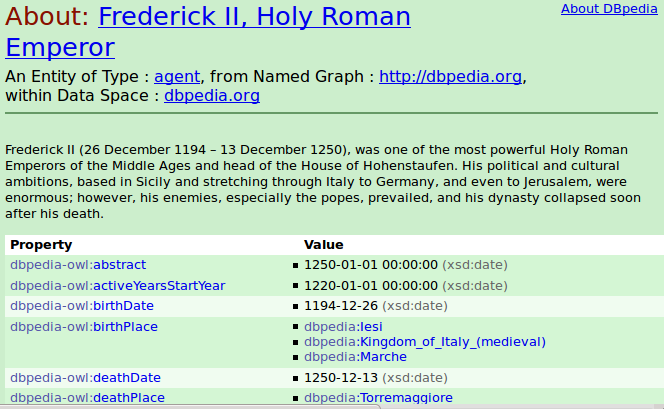
\includegraphics[width=250px]{federicoII_dbpedia.png} 
      \caption{Federico II su dbpedia.org}
  \end{figure}
\end{frame}

\begin{frame}
 \frametitle{Il Web Semantico - Tecnologie}
 
 L'insieme delle tecnologie usate nel Web Semantico costituiscono il 
 cosiddetto \emph{Semantic Web Stack}.
 
 \begin{figure}
   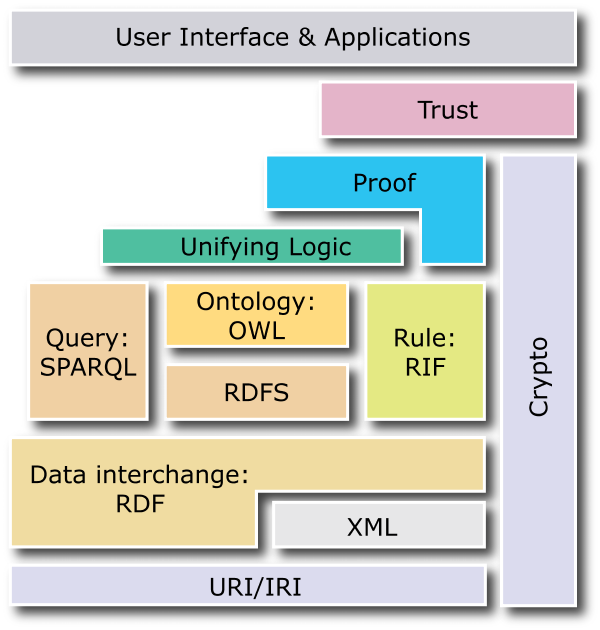
\includegraphics[width=160px]{Semantic_Web_Stack.png} 
 \end{figure}

 Il Web Semantico \`e costituito dall'insieme dei dataset 
 codificati ed esposti attraverso queste tecnologie.
\end{frame}

\begin{frame}
 \frametitle{Il Web Semantico - Linked Open Data (1/2)}
 
 Nel Web Semantico gli oggetti (concreti o astratti) sono individuati
 attraverso \emph{URI}.\footnote{In particolare IRI, vedi pi\`u avanti.}
 Questo permette di fare riferimento alla stessa entit\`a in dataset
 differenti.
 \vspace{\baselineskip}
 
 Il \emph{Linked Open Data Cloud} contiene presenti 365 dataset 
 (fonte \url{http://stats.lod2.eu/}) collegati tra loro.
\begin{figure}
    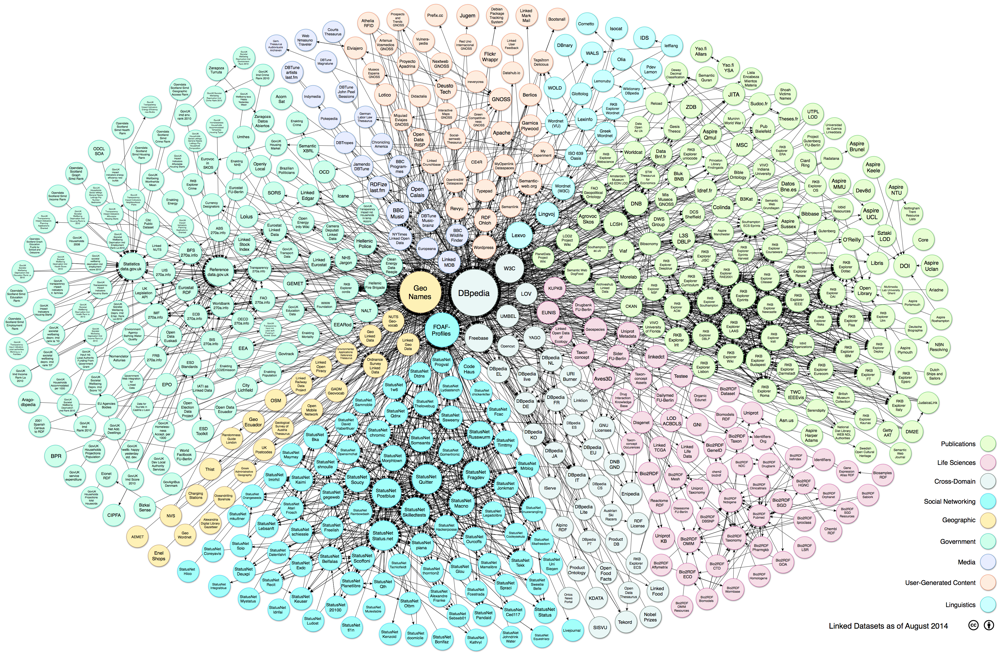
\includegraphics[width=250px]{lod-cloud_colored_1000px.png} 
    \caption{Linked Open Data Cloud}
\end{figure}
\end{frame}

\begin{frame}
 \frametitle{Il Web Semantico - Linked Open Data (2/2)}
 Alcuni dataset presenti nel Linked Open Data Cloud sono:
 
  \begin{itemize}
  \item \emph{DBPedia} (\url{dbpedia.org}) corrispondente a \url{wikipedia.org};
  \item \emph{Linked Movie Database} (\url{http://linkedmdb.org/}) controparte sul Web Semantico di \emph{Internet Movie Database} 
  (\url{http://www.imdb.com/});
  \item \emph{Linked GeoData} (\url{http://linkedgeodata.org}) 
    contiene i dati di \emph{OpenStreetMap} (\url{http://www.openstreetmap.org/});
    \item \emph{AGROVOC} (\url{http://aims.fao.org/agrovoc}) \`e il dataset della FAO (\url{http://fao.org});
    \item \emph{Europeana} (\url{http://pro.europeana.eu/linked-open-data}) contiene dati su beni culturali e tradizioni Europee. 
  \end{itemize}
\end{frame}

\section{Ontologie}

\begin{frame}
 \frametitle{Ontologie}
 
 I linguaggi di rappresentazione usati nel Web Semantico
 si basano tutti sulla nozione di \emph{ontologia}, mutuata
 dall'ambito dei sistemi di rappresentazione della conoscenza.
 \vspace{\baselineskip}

 Una \emph{ontologia} \`e una descrizione \emph{parziale} del mondo.
 Essa \`e costituita da un insieme finito di \emph{affermazioni}
 dei seguenti tipi:
 \vspace{\baselineskip}

\uncover<2->{ 
 \emph{Constraints:} impongono dei vincoli \emph{semantici} sul dominio di conoscenza 
che si va a rappresentare. La notazione richiama quella insiemistica;
\vspace{\baselineskip}
\[
 HumanBeing \Issub Mortal 
\]
}

\uncover<3->{ 
\emph{Property Assertions}: impongono una relazione tra due elementi del dominio;
\[
 Alice\,motherOf\,Bob 
\]
}

\uncover<4->{ 
\emph{Class Assertions}: indicano l'appartenenza di un elemento ad un insieme.
\[
 HumanBeing(Socrate) 
\]
}
\end{frame}

\begin{frame}
\frametitle{Ontologie - Sintassi}

Riportiamo la definizione formale per la sintassi delle ontologie.
\vspace{\baselineskip}

Siano $\CNames$, $\PNames$, $\INames$ tre insiemi infiniti, numerabili e 
a due a due disgiunti di nomi di \emph{classe}, \emph{propriet\`a} e \emph{individuo},
rispettivamente.
\vspace{\baselineskip}

Una \emph{ontologia} \`e un insieme finito di asserzioni dei seguenti tipi:
\[
 \begin{array}{ll}
  \mbox{(Constraints)} & C \Issub D\\
  & P \Issub Q \\
  & \dom(P) \Issub C \\
  & \range(P) \Issub C \\
  &\\
  \mbox{(Class Assertions)} & C(a)\\
  &\\
  \mbox{Property Assertions} & a\,P\,b\;(\mbox{equivalente }P(a,b))\\
 \end{array}
\]
dove $C, D \in \CNames$, $P, Q \in \PNames$ e $a, b \in \INames$.
\vspace{\baselineskip}

Si noti che la grammatica per i vincoli ivi riportata \`e \emph{minimale}.
Esistono linguaggi di rappresentazione che permettono di esprimere vincoli
pi\`u complessi.
\end{frame}

\begin{frame}
\frametitle{Ontologie - Sintassi}

 Segue una ontologia presentata a titolo di esempio
\[
\begin{array}{ccl}
 \Ont = & \{ & Woman \Issub Human, \\
 &&Man \Issub Human, \\
 &&Woman \Issub Female, \\
 &&Man \Issub Male, \\
 &&Woman(Alice), \\
 &&Man(Bob),\\
 &&Alice\,relative\,Bob,\\ 
 &&Alice\,child\,Charlie \}
\end{array} 
\]
\end{frame}

\begin{frame}
\frametitle{Ontologie - L'Editor Prot\'eg\'e}

  \emph{Prot\'eg\'e}\footnote{\url{http://protege.stanford.edu/products.php}} 
  \`e una suite per la modellazione di ontologie del Web Semantico, disponibile 
  sia in versione web, che in versione installabile localmente (\emph{Prot\'eg\'e Desktop}).
  \vspace{\baselineskip}

\uncover<2->{
  Permette di definire gerarchie di classi (tab \emph{Classes}) a partire dalla
  classe radice \texttt{Thing}. Per ogni classe \`e possibile definire \emph{label} 
  e \emph{comment} come annotazioni.
  \vspace{\baselineskip}
}

\uncover<3->{
  Analogamente \`e possibile definire gerarchie di propriet\`a (tab \emph{Object Poperties}) 
  a partire dalla propriet\`a radice \texttt{topObjectProperty} e di definire annotazioni
  per le propriet\`a. Inoltre, \`e possibile imporre dei vincoli di dominio e codominio
  per le propriet\`a.
  \vspace{\baselineskip}
}

\uncover<4->{
  Infine \`e possibile definire degli individui (tab \emph{Individuals}) associarli 
  a delle classi di appartenenza e metterli in relazione tra loro attraverso delle
  propriet\`a.
  \vspace{\baselineskip}
}
\end{frame}

\begin{frame}
\frametitle{Ontologie - Interpretazioni}

Per definire la semantica delle ontologie \`e necessario prima introdurre
il concetto di interpretazione. 
\vspace{\baselineskip}

Una \emph{interpretazione} $\I=(\Delta^{\I}, \cdot^{\I})$ \`e una coppia
$\Delta^{\I}$, $\cdot^{\I}$ dove:
\begin{itemize}
 \item $\Delta^{\I}$ \`e un insieme non vuoto;
 \item $\cdot^{\I}$ \`e una funzione (polimorfa) che associa
 \begin{itemize}
  \item ad ogni nome di concetto in $\CNames$ un sottoinsieme di $\Delta^{\I}$,
  \item ad ogni nome di propriet\`a in $\PNames$ una relazione su $\Delta^{\I}$,
  \item ad ogni nome di individuo in $\INames$ un elemento di $\Delta^{\I}$.
 \end{itemize}
\end{itemize}
\vspace{\baselineskip}

\uncover<2->{
 Consideriamo ad esempio la seguente ontologia
 \begin{small}
\[
\begin{array}{ccc}
 \Ont = & \{ & Woman \Issub Human, Man \Issub Human, Woman \Issub Female, Man \Issub Male, \\
 &&Woman(Alice), Man(Bob), Alice\,relative\,Bob, Alice\,child\,Charlie \}
\end{array} 
\]
 \end{small}
 Una possibile interpretazione $\I$ \`e la seguente:
 \begin{small}
\[
 \begin{array}{lcl}
    \Delta^{\I} & = & \mathbb{N}\\
    Alice^{\I} & = & 0 \\
    Bob^{\I} & = & 1 \\
    Charlie^{\I} & = & 2 \\
    Human^{\I} & = & \{ 0, 1, 2\} \\
    Male^{\I} & = & \{ 1, 2\} \\
    Female^{\I} & = & \{ 0 \} \\
    Man^{\I} & = & \{ 1, 2\} \\
    Woman^{\I} & = & \{ 0 \} \\
 \end{array}
\]
 \end{small}
 
 NB: \`e sufficiente prendere in considerazione ai nostri fini i simboli che compaiono 
 nell'ontologia.
}
\end{frame}

\begin{frame}
  \frametitle{Ontologie - Soddisfacibilit\`a}
  
  La semantica formale di cui sono equipaggiate le ontologie
  abilita l'esecuzione automatica di \emph{reasoning tasks}. Quello
  fondamentale \`e la verifica di \emph{Soddisfacibilit\`a}, che 
  permette di controllare che una ontologia non sia autocontraddittoria.
  \vspace{\baselineskip}
  
  La nozione di soddisfacibilit\`a per le ontologie \`e definita come segue.
  Sia $\I = (\Delta^{\I}, \cdot^{\I})$ una interpretazione.   
\[
\begin{array}{ccl}
 \I\mbox{ soddisfa }C \Issub D & \Longleftrightarrow & C^{\I} \subseteq D^{\I}\\  
 \I\mbox{ soddisfa }P \Issub Q & \Longleftrightarrow & P^{\I} \subseteq Q^{\I}\\  
 \I\mbox{ soddisfa }\dom(P) \Issub C & \Longleftrightarrow & (\forall [x,y] \in P^{\I})(x \in C^{\I})\\  
 \I\mbox{ soddisfa }\range(P) \Issub C & \Longleftrightarrow & (\forall [x,y] \in P^{\I})(y \in C^{\I})\\  
 \I\mbox{ soddisfa }C(a) & \Longleftrightarrow & a^{\I} \in C^{\I}\\  
 \I\mbox{ soddisfa }a\,P\,b & \Longleftrightarrow & [a^{\I}, a^{\I}] \in P^{\I}
\end{array} 
\]
per ogni $C, D \in \CNames$, $P, Q \in PNames$, $a,b \in \INames$.
\vspace{\baselineskip}

\uncover<2->{
  $\I$ soddisfa una ontologia $\Ont$ se e solo se $\I$ soddisfa tutti i vincoli e
  le asserzioni in $\Ont$.
\vspace{\baselineskip}
}

\uncover<3->{
  Una ontologia $\Ont$ \`e detta \emph{soddisfacibile} (o anche \emph{consistente}) 
  se e solo se esiste una interpretazione $\I$ che la soddisfa.
}
\end{frame}

\begin{frame}
  \frametitle{Ontologie - Soddisfacibilit\`a - Esempi (1/2)}
  
  Consideriamo la seguente ontologia
\begin{small}
\[
  \begin{array}{cll}
    \Ont = & \{ & \dom(teacherOf) \Issub Human, \\
    && Socrate\,teacherOf\,Plato \}
  \end{array} 
\]
\end{small}

Consideriamo la seguente interpretazione (di Herbrandt) $\I$: 
\begin{small}
\[
  \begin{array}{rcl}
    Socrate^{\I} & = & Socrate\\ 
    Plato^{\I} & = & Plato\\
    Human^{\I} & = & \{Socrate, Plato\}\\
    teacherOf^{\I} & = & \{ [Socrate, Plato] \}
  \end{array}
\]
\end{small}

\uncover<2->{
\[
\begin{array}{rcl}
  \I \mbox{ soddisfa }\dom(teacherOf) \Issub Human & \Longleftrightarrow & (\forall [x,y] \in teacherOf^{\I})(x \in Human^{\I})\\
  \I \mbox{ soddisfa }Socrate\,teacherOf\,Plato & \Longleftrightarrow & [Socrate,^{\I} Plato^{\I}] \in teacherOf^{\I}
\end{array}
\]

  Quindi $\I$ soddisfa $\Ont$.
}
\vspace{\baselineskip}

\uncover<3->{
  Quindi $\Ont$ \`e soddisfacibile.
}
\end{frame}

\begin{frame}
  \frametitle{Ontologie - Soddisfacibilit\`a - Esempi (2/2)}
  
  Consideriamo la seguente ontologia
\begin{small}
\[
  \begin{array}{cll}
    \Ont = & \{ & \dom(teacherOf) \Issub Human, \\
    && Socrate\,teacherOf\,Plato \}
  \end{array} 
\]
\end{small}

La seguente interpretazione (di Herbrandt) $\I_1$ NON soddisfa $\Ont$: 
\begin{small}
\[
  \begin{array}{rcl}
    Socrate^{\I_1} & = & Socrate\\ 
    Plato^{\I_1} & = & Plato\\
    Human^{\I_1} & = & \mathbf{\{Plato\}}\\
    teacherOf^{\I_1} & = & \{ [Socrate, Plato] \}
  \end{array}
\]
\end{small}

Infatti $\I_1$ non soddisfa $\dom(teacherOf) \Issub Human$ perch\`e $Socrate$ non
\`e nell'insieme $Human$ (interpretati con $\I_1$).
\end{frame}

\begin{frame}
  \frametitle{Ontologie - Implicazione}
  Date due Ontologie $\Ont$ e $\Ontp$, si dice che 
  $\Ont$ \emph{implica} $\Ontp$ se e solo se tutte le interpretazioni
  che soddisfano $\Ont$ soddisfano anche $\Ontp$. 
  \vspace{\baselineskip}  
  
\uncover<2->{
  La verifica di implicazione pu\`o essere utilizzata per ricavare
  tutte le \emph{conseguenze logiche} di una ontologia.
  \vspace{\baselineskip}
  
  \`E facile verificare che, date $\Ont$ e $\Ontp$ sotto, $\Ontp$ 
  contiene tutte le asserzioni che sono conseguenze logiche di $\Ont$.
  \vspace{\baselineskip}
  
\begin{small}
\[
  \begin{array}{clc}
    \Ont = \{ & \dom(teacherOf) \Issub Human, & \Longrightarrow \Ontp = \{ Human(Socrate) \}\\
    & Socrate\,teacherOf\,Plato \}\\
  \end{array}
\] 
\end{small}
}  
\end{frame}

\begin{frame}
  \frametitle{Ontologie - Reasoning con Prot\'eg\'e}
  L'editor Prot\'eg\'e fornisce la possibilit\`a di eseguire 
  il reasoning attraverso il men\`u \emph{Reasoner}. Le asserzioni
  inferite verranno mostrate in evidenza.
\end{frame}

\begin{frame}
  \frametitle{Ontologie nel Web Semantico}
  
  Le ontologie usate nel Web Semantico sono caratterizzate
  dai seguenti punti:
  \begin{itemize}
    \item nomi di classi, propriet\`a ed individui sono $IRI$
    \[
      IRI = \CNames \cup \PNames \cup \INames ,
    \]
    \item sono presenti dei tipi di dato \emph{concreti}.
  \end{itemize}
\end{frame}

\begin{frame}
  \frametitle{IRI nel Web Semantico}
  Nell'ambito del Web Semantico, tutti gli oggetti reali o concreti sono
  identificati attraverso IRI. As esempio
  \begin{center}
  \url{http://dbpedia.org/resource/Leonardo_da_Vinci}
  \end{center}
  \`e la IRI usata nell'ontologia \url{dbpedia.org} per indicare
  Leonardo da Vinci, e ancora 
  \begin{center}
    \begin{small}
      \url{http://data.europeana.eu/item/04802/243FA8618938F4117025F17A8B813C5F9AA4D619}
    \end{small}
  \end{center}
  indica la \emph{Mona Lisa} nell'ontologia del progetto \emph{Europeana}.
  \vspace{\baselineskip}
  
\uncover<2->{
  \emph{LodLive}\footnote{\url{http://lodlive.it}}
  e \emph{LodView}\footnote{\url{http://lodview.it}} sono due servizi online
  che permettono di navigare il Linked Open Data Cloud ed esaminare le informazioni
  in esso contenute in merito ad uno specifico elemento.
}  
\end{frame}

\begin{frame}
  \frametitle{IRI nel Web Semantico - Namespaces}
  
  Nelle ontologie del Web Semantico le IRI possono essere abbreviate
  con il meccanismo dei \emph{namespace} (prefissi), mutuato da XML.
  \vspace{\baselineskip}
  
\uncover<2->{
  Ad ogni ontologia spesso \`e assegnato un \emph{base prefix}, che solitamente
  coincide con la IRI alla quale \`e possibile scaricare l'ontologia stessa.
  Essa viene usata come prefisso per ottenere le IRI degli oggetti dell'ontologia
  nel caso in cui all'oggetto sia assegnata una IRI \emph{incompleta}. Ad esempio,
  se il base prefix dell'ontologia $\Ont$ \`e \url{http://example.org/},
  \[
   Alice \quad \Longrightarrow \mathtt{http://example.org/Alice} . 
  \]
}  

\uncover<3->{
  \`E possibile specificare degli ulteriori \emph{prefix}
  come coppie
  \[
   <prefix name> \quad \longrightarrow \quad <prefix uri> 
  \]
  e \emph{abbreviare} delle IRI nell'ontologia con la
  sintassi $<prefix name>:<IRI specific part>$. 
  \vspace{\baselineskip}
  
  Se ad
  esempio nell'ontologia \`e definito il prefisso
  \[
   ex2 \quad \longrightarrow \quad \mathtt{http://example2.org/}
  \]
  le IRI \url{ex2:Alice} verranno espanse in
  \url{http://example2.org/Alice} .
}
\end{frame}

\begin{frame}
  \frametitle{Gestione degli IRI in Prot\'eg\'e}
  
  Nell'editor Prot\'eg\'e la IRI assegnata ad ogni elemento (classe, propriet\`a,
  individuo) \`e visibile come popup che compare passando sull'elemento col mouse.
  \vspace{\baselineskip}
  
\uncover<2->{
  Nel tab \emph{Active Ontology} \`e possibile specificare la IRI dell'ontologia,
  che andrebbe usata come base prefix. Inoltre \`e possibile indicare alcuni metadati
  relativi all'ontologia stessa (autore, versione, ...).
  \vspace{\baselineskip}
}  

\uncover<3->{
  Nella sotto-tab \emph{Ontology Prefixes} \`e possibile definire ulteriori prefissi.
}  
\end{frame}

\begin{frame}
  \frametitle{Letterali}
  I letterali vengono usati per rappresentare tipi di dato \emph{concreti},
  come ad esempio stringhe di testo, numeri, date, \ldots
  \vspace{\baselineskip}

  Grazie ai letterali \`e possibile ad esempio esprimere affermazioni dei seguenti tipi:
  \begin{itemize}
  \item Il cognome di Mario \`e \emph{Rossi};
  \item Cristiano \`e nato il giorno \emph{22 Marzo 1979};
  \item L'Empire State Building \`e alto \emph{380 metri}.
  \end{itemize}
\end{frame}

\begin{frame}
  \frametitle{Datatype}
  Per introdurre i Letterali \`e necessario fornire prima la definizione di \emph{datatype}
  (vedi \url{http://www.w3.org/TR/2014/REC-rdf11-concepts-20140225/\#section-Datatypes} e 
  \url{http://www.w3.org/TR/xmlschema11-2/}).
  \vspace{\baselineskip}

  Un \emph{datatype} \`e caratterizzato da tre componenti:
  \begin{itemize}
    \item un \emph{lexical space}, ossia un insieme di stringhe (finite) di caratteri nella codifica \emph{UNICODE};
    \item un \emph{value space}, che \`e un insieme non meglio specificato e numerabile di \emph{valori} (interi, date,
    Booleani, \ldots);
    \item un \emph{lexical-value mapping} che associa ad ogni stringa nel lexical space un elemento nel value space.
  \end{itemize}
  \vspace{\baselineskip}

  I datatype vengono di solito indicati con delle IRI.
\end{frame}

\begin{frame}
  \frametitle{Datatype - Esempio 1 : \url{xsd:integer}}
  Il datatype \url{xsd:integer} (dove \url{xsd} \`e l'abbreviazione per il namespace \url{http://www.w3.org/2001/XMLSchema\#})
  \`e definito come segue:

  \begin{itemize}
    \item il \emph{lexical space} di \url{xsd:integer} \`e costituito da tutte le sequenze finite di cifre da 0 a 9, possibilmente
    precedute dal carattere ``-'' o ``+'';
    \item il \emph{value space} \`e l'insieme dei numeri interi;
    \item il valore di una stringa nel lexical space di \url{xsd:integer} si ottiene considerando le cifre 
    presenti nella stringa come cifre del corrispondente numero in base $10$, e moltiplicando il numero cos\`i ottenuto per
    $-1$ nel caso in cui la stringa inizi con il carattere ``-''.
  \end{itemize}
\end{frame}

\begin{frame}
  \frametitle{Datatype - Esempio 2 : \url{xsd:string}}
  Il datatype \url{xsd:string} \`e definito come segue:

  \begin{itemize}
    \item il \emph{lexical space} di \url{xsd:string} comprende 
    tutte le sequenze di caratteri (UNICODE) di zero o pi\`u caratteri;
    \item il \emph{value space} di \url{xsd:string} coincide col suo 
    lexical space;
    \item il \emph{lexical-value mapping} associa ogni stringa nel lexical space
    con se stessa (indetit\'a).
  \end{itemize}
\end{frame}

\begin{frame}
  \frametitle{Altri esempi di datatype}
  Riportiamo alcuni datatype (mutuati da XML Schema) di uso comune.

  \begin{small}
    \begin{tabular}{|l|l|}
    \hline
    \url{xsd:boolean} & true, false\\
    \url{xsd:decimal} & Arbitrary-precision decimal numbers\\
    \url{xsd:integer} & Arbitrary-size integer numbers\\
    \url{xsd:double} & 64-bit floating point numbers incl. ±Inf, ±0, NaN\\
    \url{xsd:float} & 32-bit floating point numbers incl. ±Inf, ±0, NaN\\
    \url{xsd:date} & Dates (yyyy-mm-dd) with or without timezone\\
    \url{xsd:time} & Times (hh:mm:ss.sss…) with or without timezone\\
    \url{xsd:dateTime} & Date and time with or without timezone\\
    \url{xsd:dateTimeStamp} & Date and time with required timezone\\
    \url{xsd:duration} & Duration of time\\
    \url{xsd:byte} & -128\ldots+127 (8 bit)\\
    \url{xsd:short} & -32768\ldots+32767 (16 bit) \\
    \url{xsd:int} & -2147483648\ldots+2147483647 (32 bit)\\
    \url{xsd:long} & -9223372036854775808\ldots+9223372036854775807 (64 bit)\\
    \url{xsd:unsignedByte} & 0\ldots255 (8 bit)\\
    \url{xsd:unsignedShort} & 0\ldots65535 (16 bit)\\
    \url{xsd:unsignedInt} & 0\ldots4294967295 (32 bit)\\
    \url{xsd:unsignedLong} & 0\ldots18446744073709551615 (64 bit)\\
    \url{xsd:positiveInteger} & Integer numbers $>0$\\
    \url{xsd:nonNegativeInteger} & Integer numbers $\geq 0$\\
    \url{xsd:negativeInteger} & Integer numbers $<0$\\
    \url{xsd:nonPositiveInteger} & Integer numbers $\leq 0$\\
    \url{xsd:hexBinary} & Hex-encoded binary data\\
    \hline
    \end{tabular}
  \end{small}
\end{frame}

\begin{frame}
  \frametitle{Letterali - Definizione}
  Formalmente, i letterali sono definiti come segue (vedi 
  \url{http://www.w3.org/TR/2014/REC-rdf11-concepts-20140225/\#section-Graph-Literal}).
  \vspace{\baselineskip}

  Un \emph{letterale} \`e costituito da un \emph{datatype} $t$ e da una 
  stringa di caratteri nel lexical space di $t$ (la cosiddetta \emph{lexical form}
  del letterale).
  \vspace{\baselineskip}

  Se un letterale \`e di tipo \url{xsd:string}, ad esso pu\`o essere associato un
  \emph{language tag} ad indicarne la \emph{lingua}. Per i valori che questo attributo pu\`o
  assumere fare riferimento allo \emph{IANA Language Subtag Registry}.
\end{frame}

\begin{frame}
\frametitle{Letterali - Esempi}
  Seguono alcuni esempi di letterali:

  \begin{center}
  \begin{tabular}{|l|l|c|}
    \hline
    \textbf{lexical form} & \textbf{data type} & \textbf{language tag}\\
    \hline
    ``380'' & \url{xsd:integer} & - \\
    ``March-22-1979'' & \url{xsd:date} & - \\
    ``Rossi'' & \url{xsd:string} & - \\
    ``Parigi'' & \url{xsd:string} & it \\
    ``Paris'' & \url{xsd:string} & en\\
    \hline
  \end{tabular}
  \end{center}
  \vspace{\baselineskip}

  Nel caso in cui si ometta l'indicazione del tipo di dato, il letterale si assume essere
  di tipo \url{xsd:string}.
\end{frame}


\begin{frame}
  \frametitle{Letterali - Notazione (1/3)}
  Per indicare i letterali spesso si usano le seguenti notazioni
  \[
  \begin{array}{c}
    \literal{lexform}{type} \\
    \\
    < lexform, type >
  \end{array}
  \]
  ove $lexform$ e $type$ sono la lexical form e il data type del letterale, rispettivamente.
  \vspace{\baselineskip}

  Alcuni esempi:
  \[
  \begin{array}{ll}
    \literal{380}{xsd:integer} & <``380'', xsd:integer>\\
    \literal{March-22-1979}{xsd:date} & <``March-22-1979'', xsd:date>\\
    \literal{Rossi}{xsd:string} & <``Rossi'', xsd:string>
  \end{array}
  \]
\end{frame}

\begin{frame}
\frametitle{Letterali - Notazione (2/3)}
  Nel seguito indicheremo con 
  \begin{itemize}
    \item $\datatypes$ l'insieme di tutti i possibili data type,
  e con
    \item $\literals$ l'insieme dei letterali.
  \end{itemize}
  \vspace{\baselineskip}

  Si assume per convenienza 
  che i data type dei letterali in $\literals$ siano tutti 
  contenuti in $\datatypes$.
\end{frame}

\newcommand{\mathurl}[1]{\mbox{\url{#1}}}

\begin{frame}
  \frametitle{Letterali - Notazione (3/3)}
  Inoltre, dato un letterale $l \in \literals$, indicheremo con
  \begin{itemize}
    \item $datatype(l)$ il tipo di dato di $l$ (ovviamente $datatype(l) \in \datatypes$), e con 
    \item $lexform(l)$ la lexical form di $l$.
  \end{itemize}
  \vspace{\baselineskip}

  Seguono alcuni esempi:
  \[
  \begin{array}{l}
    datatype(\literal{380}{xsd:integer}) = \mathurl{xsd:integer}\\
    datatype(\literal{March-22-1979}{xsd:date}) = \mathurl{xsd:date}\\
    datatype(\literal{Rossi}{xsd:string}) = \mathurl{xsd:string}\\
    \\
    lexform(\literal{380}{xsd:integer}) = \stringLiteral{380}\\
    lexform(\literal{March-22-1979}{xsd:date}) = \stringLiteral{March-22-1979}\\
    lexform(\literal{Rossi}{xsd:string}) = \stringLiteral{Rossi} 
  \end{array}
  \]
\end{frame}


\begin{frame}
\frametitle{Confronto tra Letterali}
  Due letterali sono uguali se e solo se sono uguali le loro lexical form,
  se hanno lo stesso tipo e se sono uguali i loro language tag, ove presenti.
  Di conseguenza due letterali possono essere diversi anche avendo lo stesso
  \emph{valore}. Ad esempio i due seguenti letterali hanno entrambi 
  come valore l'intero $1$ ma sono diversi:
  \vspace{\baselineskip}

  \[
  \begin{array}{l}
    \literal{1}{xsd:integer}\\
    \literal{01}{xsd:integer} .\\
  \end{array}
  \]
\end{frame}

\begin{frame}
 \frametitle{Ontologie - Datatype Properties}
 \`E possibile definire delle propriet\`a che abbiano un oggetto
 di tipo concreto (su Prot\'eg\'e la tab \emph{Datatype properties}).
 \vspace{\baselineskip}
 
% \uncover<2->{ 
 \`E possibile vincolare una propriet\`a  ad avere come codominio
 solo letterali con un certo data type. 
 \vspace{\baselineskip}
  
 Alcuni esempi vincoli di questa natura sono
 \[
 \begin{array}{l}
    \range(surname) \Issub \mathurl{xsd:string} \\
    \range(hasbirth) \Issub \mathurl{xsd:date}\\
 \end{array}
 \]
  con $surname, hasbirth \in \PNames$ e 
  \url{xsd:string}, \url{xsd:date} data type.
% }
\end{frame}

\end{document}
